\section{Algorytm}
\label{sec_algorytm}

\subsection{Założenia}
\label{subsec_zalozenia}

Idee metody Naiwnego Bayesa można łatwo wyjaśnić na prostym przykładzie, precyzyjny opis matematyczny został zamieszczony w rozdziale \ref{sec_opis_mat}. Na rysunku \ref{fig_bayes_przyklad} przedstawiony został zbiór punktów, podzielony na dwie klasy (czerwone i zielone). Zadaniem klasyfikatora jest przydzielenie nowego obiektu do jednej z tych klas. W tym przypadku klasyfikacja będzie dokonana na podstawie położenia i elementów znajdujących się w sąsiedztwie nowo dodanego obiektu. Podany zbiór punktów, pełni w tym przypadku rolę zbioru uczącego.

\begin{figure}[!htb]
  \begin{center}
    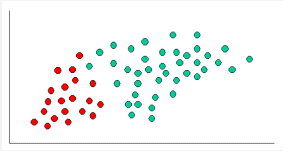
\includegraphics[scale = 1]
    {img/bayes_przyklad.png}
  \end{center}
  \caption{Prosty przykład - zbiór punktów (źródło \ref{})}
  \label{fig_bayes_przyklad}
\end{figure}

\subsection{Klasyfikacja}
\label{subsec_klasyfikacja}

W omawianym przykładzie możemy zauważyć, że obiektów zielonych jest dwa razy więcej niż czerwonych. W związku z tym możemy założyć ''z góry'', że nowy obiekt ma dwa razy większe prawdopodobieństwo bycia zielonym niż czerwonym. Obliczone w ten sposób prawdopodobieństwo nazywane jest prawdopodobieństwem \textit{a priori}. 

Wszystkich obiektów jest 60 w czym 40 zielonych i 20 czerwonych. Prawdopodobieństwo \textit{a priori} wylicza się jako iloraz liczby obiektów danego koloru do liczby wszystkich obiektów. Następnie przystępujemy do kolejnego etapu klasyfikacji, przyjmijmy pewne sąsiedztwo nowego punktu (rysunek \ref{fig_bayes_przyklad2}). Możemy założyć, że im więcej obiektów danego koloru w otoczeniu nowego obiektu, tym bardziej prawdopodobne, że jest on tego koloru. Wyznaczone w ten sposób prawdopodobieństwo nazywane jest szansą, oblicza się je jako stosunek liczby obiektów danego koloru w sąsiedztwie, do całkowitej liczby obiektów tego koloru.

\begin{figure}[!htb]
  \begin{center}
    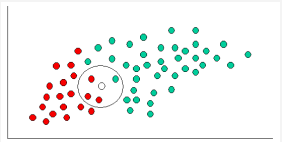
\includegraphics[scale = 1]
    {img/bayes_przyklad_2.png}
  \end{center}
  \caption{Prosty przykład - sąsiedztwo (źródło \ref{})}
  \label{fig_bayes_przyklad2}
\end{figure}

Mając dane prawdopodobieństwo \textit{a priori} oraz szansę, możemy przystąpić do ostatniego etapu klasyfikacji. Końcowe prawdopodobieństwo czy nowy obiekt należy do danej klasy (jest danego koloru) obliczane jest jako iloczyn dwóch wyznaczonych wcześniej prawdopodobieństw. Zostaje on oczywiście przypisany do klasy o większym prawdopodobieństwie.


\subsection{Wykorzystanie w detekcji pulsu}
\label{subsec_bayes_detekcja_pulsu}

Omówiony w poprzednich punktach przykład, był bardzo uproszczony i miał na celu jedynie pokazać idee klasyfikatora. Klasyfikacja zespołu QRS jest problemem wielowymiarowym (dokładnie 18 wymiarowym, gdyż jest to rozmiar wektora cech). W takim przypadku nieco inaczej oblicza ''szansa''. Obliczane jest osobno prawdopodobieństwo przynależności do danej klasy na podstawie każdego elementu z wektora cech. Ostatecznie pod uwagę brany jest iloczyn wszystkich prawdopodobieństw.

Kolejnym zagadnieniem jest sposób obliczania prawdopodobieństwa na podstawie cechy. W przypadku niniejszego projektu wykorzystywany jest w tym celu rozkład normalny (rozdział \ref{sec_rozklady}). Dla każdej klasy, poszczególne cechy mają przypisaną wartość średnią i odchylenie standardowe. Są one obliczane na podstawie zbioru uczącego w trakcie procesu uczenia.

\subsection{Zbiór testowy i uczący}
\label{subsec_test_ucz}

